% Graphic for TeX using PGF
% Title: /home/braulio/PycharmProjects/TFG/doc/clases.dia
% Creator: Dia v0.97.3
% CreationDate: Mon Sep  4 20:42:15 2017
% For: braulio
% \usepackage{tikz}
% The following commands are not supported in PSTricks at present
% We define them conditionally, so when they are implemented,
% this pgf file will use them.
\ifx\du\undefined
  \newlength{\du}
\fi
\setlength{\du}{15\unitlength}
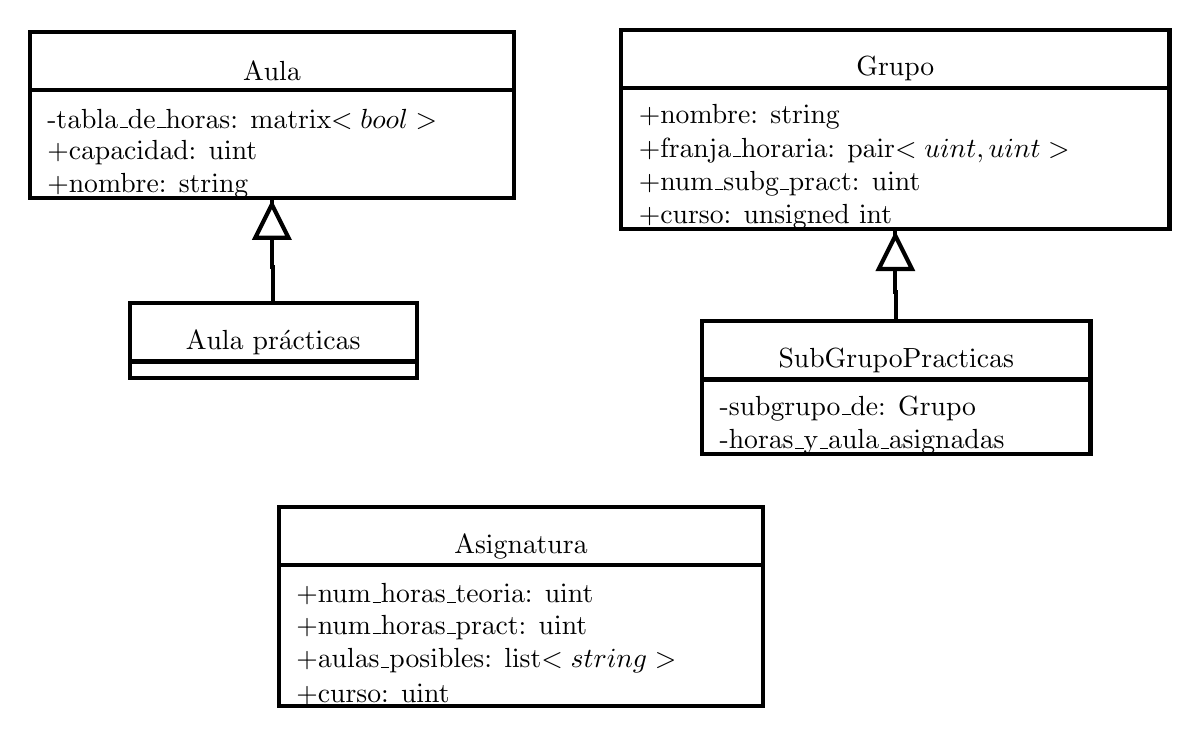
\begin{tikzpicture}
\pgftransformxscale{1.000000}
\pgftransformyscale{-1.000000}
\definecolor{dialinecolor}{rgb}{0.000000, 0.000000, 0.000000}
\pgfsetstrokecolor{dialinecolor}
\definecolor{dialinecolor}{rgb}{1.000000, 1.000000, 1.000000}
\pgfsetfillcolor{dialinecolor}
\pgfsetlinewidth{0.100000\du}
\pgfsetdash{}{0pt}
\definecolor{dialinecolor}{rgb}{1.000000, 1.000000, 1.000000}
\pgfsetfillcolor{dialinecolor}
\fill (12.350000\du,4.800000\du)--(12.350000\du,6.200000\du)--(24.015000\du,6.200000\du)--(24.015000\du,4.800000\du)--cycle;
\definecolor{dialinecolor}{rgb}{0.000000, 0.000000, 0.000000}
\pgfsetstrokecolor{dialinecolor}
\draw (12.350000\du,4.800000\du)--(12.350000\du,6.200000\du)--(24.015000\du,6.200000\du)--(24.015000\du,4.800000\du)--cycle;
% setfont left to latex
\definecolor{dialinecolor}{rgb}{0.000000, 0.000000, 0.000000}
\pgfsetstrokecolor{dialinecolor}
\node at (18.182500\du,5.750000\du){Aula};
\definecolor{dialinecolor}{rgb}{1.000000, 1.000000, 1.000000}
\pgfsetfillcolor{dialinecolor}
\fill (12.350000\du,6.200000\du)--(12.350000\du,8.800000\du)--(24.015000\du,8.800000\du)--(24.015000\du,6.200000\du)--cycle;
\definecolor{dialinecolor}{rgb}{0.000000, 0.000000, 0.000000}
\pgfsetstrokecolor{dialinecolor}
\draw (12.350000\du,6.200000\du)--(12.350000\du,8.800000\du)--(24.015000\du,8.800000\du)--(24.015000\du,6.200000\du)--cycle;
% setfont left to latex
\definecolor{dialinecolor}{rgb}{0.000000, 0.000000, 0.000000}
\pgfsetstrokecolor{dialinecolor}
\node[anchor=west] at (12.500000\du,6.900000\du){-tabla\_de\_horas: matrix$<bool>$};
% setfont left to latex
\definecolor{dialinecolor}{rgb}{0.000000, 0.000000, 0.000000}
\pgfsetstrokecolor{dialinecolor}
\node[anchor=west] at (12.500000\du,7.700000\du){+capacidad: uint};
% setfont left to latex
\definecolor{dialinecolor}{rgb}{0.000000, 0.000000, 0.000000}
\pgfsetstrokecolor{dialinecolor}
\node[anchor=west] at (12.500000\du,8.500000\du){+nombre: string};
\pgfsetlinewidth{0.100000\du}
\pgfsetdash{}{0pt}
\definecolor{dialinecolor}{rgb}{1.000000, 1.000000, 1.000000}
\pgfsetfillcolor{dialinecolor}
\fill (14.756600\du,11.342000\du)--(14.756600\du,12.742000\du)--(21.669100\du,12.742000\du)--(21.669100\du,11.342000\du)--cycle;
\definecolor{dialinecolor}{rgb}{0.000000, 0.000000, 0.000000}
\pgfsetstrokecolor{dialinecolor}
\draw (14.756600\du,11.342000\du)--(14.756600\du,12.742000\du)--(21.669100\du,12.742000\du)--(21.669100\du,11.342000\du)--cycle;
% setfont left to latex
\definecolor{dialinecolor}{rgb}{0.000000, 0.000000, 0.000000}
\pgfsetstrokecolor{dialinecolor}
\node at (18.212850\du,12.292000\du){Aula prácticas};
\definecolor{dialinecolor}{rgb}{1.000000, 1.000000, 1.000000}
\pgfsetfillcolor{dialinecolor}
\fill (14.756600\du,12.742000\du)--(14.756600\du,13.142000\du)--(21.669100\du,13.142000\du)--(21.669100\du,12.742000\du)--cycle;
\definecolor{dialinecolor}{rgb}{0.000000, 0.000000, 0.000000}
\pgfsetstrokecolor{dialinecolor}
\draw (14.756600\du,12.742000\du)--(14.756600\du,13.142000\du)--(21.669100\du,13.142000\du)--(21.669100\du,12.742000\du)--cycle;
\pgfsetlinewidth{0.100000\du}
\pgfsetdash{}{0pt}
\pgfsetmiterjoin
\pgfsetbuttcap
{
\definecolor{dialinecolor}{rgb}{0.000000, 0.000000, 0.000000}
\pgfsetfillcolor{dialinecolor}
% was here!!!
\definecolor{dialinecolor}{rgb}{0.000000, 0.000000, 0.000000}
\pgfsetstrokecolor{dialinecolor}
\draw (18.182500\du,8.850250\du)--(18.182500\du,10.470893\du)--(18.212850\du,10.470893\du)--(18.212850\du,11.291536\du);
}
\definecolor{dialinecolor}{rgb}{0.000000, 0.000000, 0.000000}
\pgfsetstrokecolor{dialinecolor}
\draw (18.182500\du,9.762054\du)--(18.182500\du,10.470893\du)--(18.212850\du,10.470893\du)--(18.212850\du,11.291536\du);
\pgfsetmiterjoin
\definecolor{dialinecolor}{rgb}{1.000000, 1.000000, 1.000000}
\pgfsetfillcolor{dialinecolor}
\fill (18.582500\du,9.762054\du)--(18.182500\du,8.962054\du)--(17.782500\du,9.762054\du)--cycle;
\pgfsetlinewidth{0.100000\du}
\pgfsetdash{}{0pt}
\pgfsetmiterjoin
\definecolor{dialinecolor}{rgb}{0.000000, 0.000000, 0.000000}
\pgfsetstrokecolor{dialinecolor}
\draw (18.582500\du,9.762054\du)--(18.182500\du,8.962054\du)--(17.782500\du,9.762054\du)--cycle;
% setfont left to latex
\pgfsetlinewidth{0.100000\du}
\pgfsetdash{}{0pt}
\definecolor{dialinecolor}{rgb}{1.000000, 1.000000, 1.000000}
\pgfsetfillcolor{dialinecolor}
\fill (26.600000\du,4.750000\du)--(26.600000\du,6.150000\du)--(39.805000\du,6.150000\du)--(39.805000\du,4.750000\du)--cycle;
\definecolor{dialinecolor}{rgb}{0.000000, 0.000000, 0.000000}
\pgfsetstrokecolor{dialinecolor}
\draw (26.600000\du,4.750000\du)--(26.600000\du,6.150000\du)--(39.805000\du,6.150000\du)--(39.805000\du,4.750000\du)--cycle;
% setfont left to latex
\definecolor{dialinecolor}{rgb}{0.000000, 0.000000, 0.000000}
\pgfsetstrokecolor{dialinecolor}
\node at (33.202500\du,5.700000\du){Grupo};
\definecolor{dialinecolor}{rgb}{1.000000, 1.000000, 1.000000}
\pgfsetfillcolor{dialinecolor}
\fill (26.600000\du,6.150000\du)--(26.600000\du,9.550000\du)--(39.805000\du,9.550000\du)--(39.805000\du,6.150000\du)--cycle;
\definecolor{dialinecolor}{rgb}{0.000000, 0.000000, 0.000000}
\pgfsetstrokecolor{dialinecolor}
\draw (26.600000\du,6.150000\du)--(26.600000\du,9.550000\du)--(39.805000\du,9.550000\du)--(39.805000\du,6.150000\du)--cycle;
% setfont left to latex
\definecolor{dialinecolor}{rgb}{0.000000, 0.000000, 0.000000}
\pgfsetstrokecolor{dialinecolor}
\node[anchor=west] at (26.750000\du,6.850000\du){+nombre: string};
% setfont left to latex
\definecolor{dialinecolor}{rgb}{0.000000, 0.000000, 0.000000}
\pgfsetstrokecolor{dialinecolor}
\node[anchor=west] at (26.750000\du,7.650000\du){+franja\_horaria: pair$<uint, uint>$};
% setfont left to latex
\definecolor{dialinecolor}{rgb}{0.000000, 0.000000, 0.000000}
\pgfsetstrokecolor{dialinecolor}
\node[anchor=west] at (26.750000\du,8.450000\du){+num\_subg\_pract: uint};
% setfont left to latex
\definecolor{dialinecolor}{rgb}{0.000000, 0.000000, 0.000000}
\pgfsetstrokecolor{dialinecolor}
\node[anchor=west] at (26.750000\du,9.250000\du){+curso: unsigned int};
\pgfsetlinewidth{0.100000\du}
\pgfsetdash{}{0pt}
\definecolor{dialinecolor}{rgb}{1.000000, 1.000000, 1.000000}
\pgfsetfillcolor{dialinecolor}
\fill (18.350000\du,16.250000\du)--(18.350000\du,17.650000\du)--(30.015000\du,17.650000\du)--(30.015000\du,16.250000\du)--cycle;
\definecolor{dialinecolor}{rgb}{0.000000, 0.000000, 0.000000}
\pgfsetstrokecolor{dialinecolor}
\draw (18.350000\du,16.250000\du)--(18.350000\du,17.650000\du)--(30.015000\du,17.650000\du)--(30.015000\du,16.250000\du)--cycle;
% setfont left to latex
\definecolor{dialinecolor}{rgb}{0.000000, 0.000000, 0.000000}
\pgfsetstrokecolor{dialinecolor}
\node at (24.182500\du,17.200000\du){Asignatura};
\definecolor{dialinecolor}{rgb}{1.000000, 1.000000, 1.000000}
\pgfsetfillcolor{dialinecolor}
\fill (18.350000\du,17.650000\du)--(18.350000\du,21.050000\du)--(30.015000\du,21.050000\du)--(30.015000\du,17.650000\du)--cycle;
\definecolor{dialinecolor}{rgb}{0.000000, 0.000000, 0.000000}
\pgfsetstrokecolor{dialinecolor}
\draw (18.350000\du,17.650000\du)--(18.350000\du,21.050000\du)--(30.015000\du,21.050000\du)--(30.015000\du,17.650000\du)--cycle;
% setfont left to latex
\definecolor{dialinecolor}{rgb}{0.000000, 0.000000, 0.000000}
\pgfsetstrokecolor{dialinecolor}
\node[anchor=west] at (18.500000\du,18.350000\du){+num\_horas\_teoria: uint};
% setfont left to latex
\definecolor{dialinecolor}{rgb}{0.000000, 0.000000, 0.000000}
\pgfsetstrokecolor{dialinecolor}
\node[anchor=west] at (18.500000\du,19.150000\du){+num\_horas\_pract: uint};
% setfont left to latex
\definecolor{dialinecolor}{rgb}{0.000000, 0.000000, 0.000000}
\pgfsetstrokecolor{dialinecolor}
\node[anchor=west] at (18.500000\du,19.950000\du){+aulas\_posibles: list$<string>$};
% setfont left to latex
\definecolor{dialinecolor}{rgb}{0.000000, 0.000000, 0.000000}
\pgfsetstrokecolor{dialinecolor}
\node[anchor=west] at (18.500000\du,20.750000\du){+curso: uint};
\pgfsetlinewidth{0.100000\du}
\pgfsetdash{}{0pt}
\definecolor{dialinecolor}{rgb}{1.000000, 1.000000, 1.000000}
\pgfsetfillcolor{dialinecolor}
\fill (28.547000\du,11.775000\du)--(28.547000\du,13.175000\du)--(37.902000\du,13.175000\du)--(37.902000\du,11.775000\du)--cycle;
\definecolor{dialinecolor}{rgb}{0.000000, 0.000000, 0.000000}
\pgfsetstrokecolor{dialinecolor}
\draw (28.547000\du,11.775000\du)--(28.547000\du,13.175000\du)--(37.902000\du,13.175000\du)--(37.902000\du,11.775000\du)--cycle;
% setfont left to latex
\definecolor{dialinecolor}{rgb}{0.000000, 0.000000, 0.000000}
\pgfsetstrokecolor{dialinecolor}
\node at (33.224500\du,12.725000\du){SubGrupoPracticas};
\definecolor{dialinecolor}{rgb}{1.000000, 1.000000, 1.000000}
\pgfsetfillcolor{dialinecolor}
\fill (28.547000\du,13.175000\du)--(28.547000\du,14.975000\du)--(37.902000\du,14.975000\du)--(37.902000\du,13.175000\du)--cycle;
\definecolor{dialinecolor}{rgb}{0.000000, 0.000000, 0.000000}
\pgfsetstrokecolor{dialinecolor}
\draw (28.547000\du,13.175000\du)--(28.547000\du,14.975000\du)--(37.902000\du,14.975000\du)--(37.902000\du,13.175000\du)--cycle;
% setfont left to latex
\definecolor{dialinecolor}{rgb}{0.000000, 0.000000, 0.000000}
\pgfsetstrokecolor{dialinecolor}
\node[anchor=west] at (28.697000\du,13.875000\du){-subgrupo\_de: Grupo};
% setfont left to latex
\definecolor{dialinecolor}{rgb}{0.000000, 0.000000, 0.000000}
\pgfsetstrokecolor{dialinecolor}
\node[anchor=west] at (28.697000\du,14.675000\du){-horas\_y\_aula\_asignadas};
\pgfsetlinewidth{0.100000\du}
\pgfsetdash{}{0pt}
\pgfsetmiterjoin
\pgfsetbuttcap
{
\definecolor{dialinecolor}{rgb}{0.000000, 0.000000, 0.000000}
\pgfsetfillcolor{dialinecolor}
% was here!!!
\definecolor{dialinecolor}{rgb}{0.000000, 0.000000, 0.000000}
\pgfsetstrokecolor{dialinecolor}
\draw (33.202500\du,9.600299\du)--(33.202500\du,11.062448\du)--(33.224500\du,11.062448\du)--(33.224500\du,11.724597\du);
}
\definecolor{dialinecolor}{rgb}{0.000000, 0.000000, 0.000000}
\pgfsetstrokecolor{dialinecolor}
\draw (33.202500\du,10.512102\du)--(33.202500\du,11.062448\du)--(33.224500\du,11.062448\du)--(33.224500\du,11.724597\du);
\pgfsetmiterjoin
\definecolor{dialinecolor}{rgb}{1.000000, 1.000000, 1.000000}
\pgfsetfillcolor{dialinecolor}
\fill (33.602500\du,10.512102\du)--(33.202500\du,9.712102\du)--(32.802500\du,10.512102\du)--cycle;
\pgfsetlinewidth{0.100000\du}
\pgfsetdash{}{0pt}
\pgfsetmiterjoin
\definecolor{dialinecolor}{rgb}{0.000000, 0.000000, 0.000000}
\pgfsetstrokecolor{dialinecolor}
\draw (33.602500\du,10.512102\du)--(33.202500\du,9.712102\du)--(32.802500\du,10.512102\du)--cycle;
% setfont left to latex
\end{tikzpicture}
